\section{Odometry}\label{sec:visual-odometry}
As introduced in \hyperref[sec:the-problem]{\S1.2}, the problem of odometry is about the estimation of the change in a robot's pose over time.

The odometry, also known as self-localization, can be classified in different ways, in the next section, there is a more detailed description of the different types of odometry.

\subsection{Taxonomy}\label{subsec:tassonomy}
There different types of odometry, which based on the classification of Alkendi et al.~\cite{vo_state_of_art} can be divided into two main categories: \gls{gnss} available and GNSS not available.
\begin{figure}[H]
    \centering
    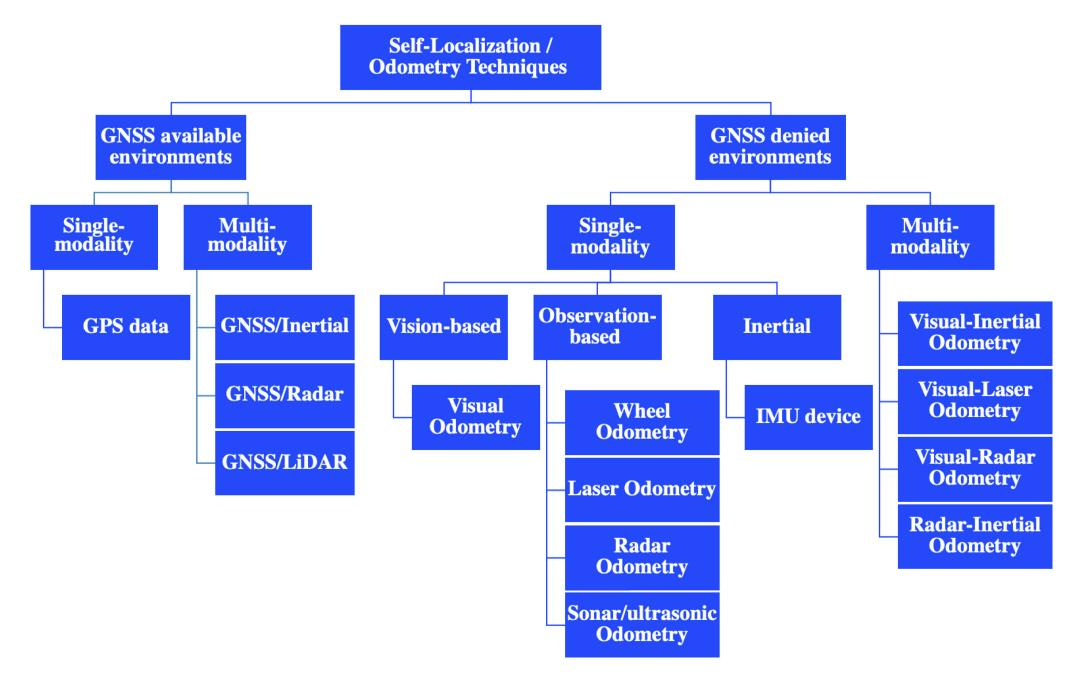
\includegraphics[width=\textwidth]{images/2_2_taxonomy_odometry}
    \caption{Taxonomy of odometry techniques.}\label{fig:odometry-taxonomy}
\end{figure}
The main difference between the left-branch and the right branch is that in the left one, the systems can use the Global Navigation Satellite System (GNSS) to get the position of the robot, while in the right one, the systems cannot use the GNSS, so the task is much more difficult.
Then, for the right branch, there are two classes, the first one is \textit{Single modality} meanwhile the other is about the combination of different modalities.
Finally, the \textit{Single modality} can be divided into three classes, the first one is \textit{Vision-based}, second one is \textit{Observation based} and the last is \textit{Inertial}.
The difference between first two are is that the first is about visual information, i.e., images, while the second one is about the information from the sensors, i.e., the laser scanner, radar sensor and sonar sensor.

The visual odometry, then, can be divided in many categories, like in the following figure.

\begin{figure}[H]
    \centering
    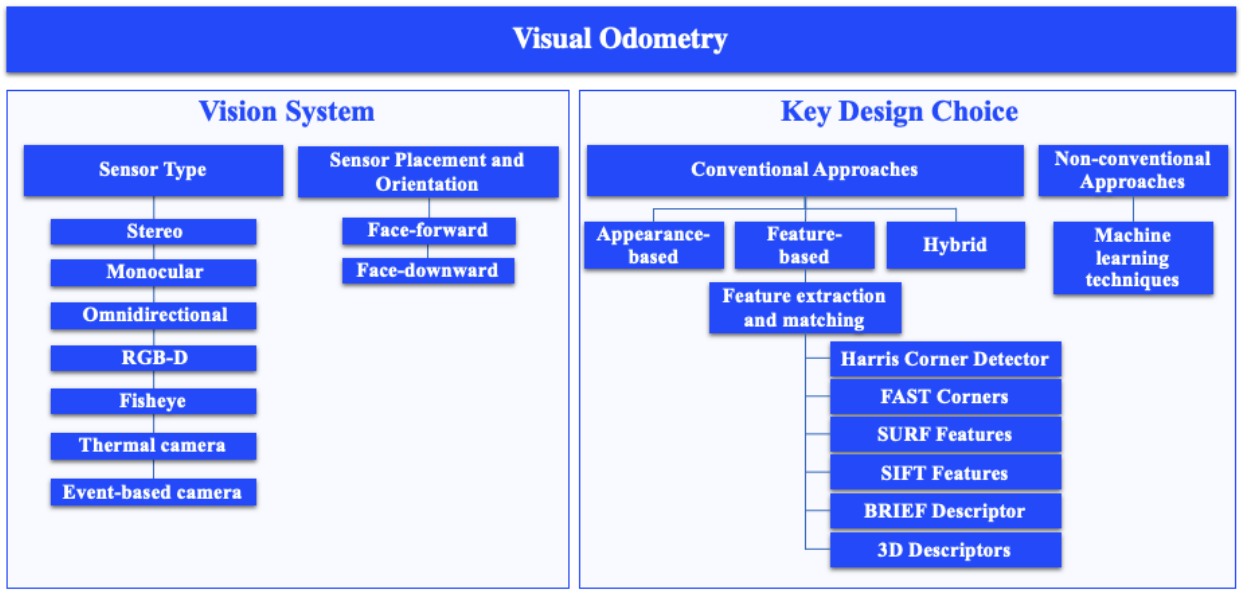
\includegraphics[width=\textwidth]{images/2_2_visual_odometry_taxonomy}
    \caption{Taxonomy of visual odometry techniques proposed in the literature.}\label{fig:visual-odometry-taxonomy}
\end{figure}
Our solution will be a monocular, face-forward, non-conventional approach by using machine learning technique, in particular, a neural network based on transformer model.

\subsection{Reference systems}\label{subsec:reference-systems}
To tackle the problem of odometry, we need as to choose the representation system to adopt.
There are many way of representing the pose of the camera or the robot, but the most common are the \textit{Euler angles}, \textit{roto-translation matrix}, \textit{quaternions} and \textit{homogeneous coordinates}.
In the project we will use the first twos, the \textit{Euler angles} and the \textit{roto-transformation matrix}.
The KITTI dataset provides the pose of the camera in the \textit{roto-transformation matrix} format flattened into a list of 12 numbers.

\subsubsection*{Euler angles}
The Euler angles (\cite{euler_angles}) are introduced by Euler to describe the orientation of a rigid body with respect to a fixed coordinate system.
According to Euler's rotation theorem, any rotation may be described using three angles.
If the rotations are written in terms of rotation matrices \textbf{D}, \textbf{C} and \textbf{B}, then, a general rotation \textbf{A} can be written as:
\begin{equation}
    \textbf{A} = \textbf{D} \textbf{C} \textbf{B}
    \label{eq:general_rotation}
\end{equation}
where $D$, $C$ and $B$ are called Euler angles.
There are several conventions for Euler Angles, depending on the axes about which the rotation are carried out.
Write the matrix \textbf{A} as:
\begin{equation}
    \textbf{A} = \begin{bmatrix}
                     a_{11} & a_{12} & a_{13} \\
                     a_{21} & a_{22} & a_{23} \\
                     a_{31} & a_{32} & a_{33}
    \end{bmatrix}
    \label{eq:matrix_A}
\end{equation}
The so-called ``x-convention'' is the most common one, in this convention, the rotation given by angles ($\phi$, $\theta$, $\psi$) respectively for \textit{roll}, \textit{pitch} and \textit{yaw} is defined as:
\begin{enumerate}
    \item by an angle $\phi$ about the $z$-axis using $D$;
    \item then, by an angle $\theta \in [0,\pi]$ about the former $x$-axis using $C$;
    \item third rotation is by an angle $\psi$ about the former $z$-axis using $B$.
\end{enumerate}
Here, we have a graphical example of the \textit{roll}, \textit{pitch} and \textit{yaw} axis:
\begin{figure}[H]
    \centering
    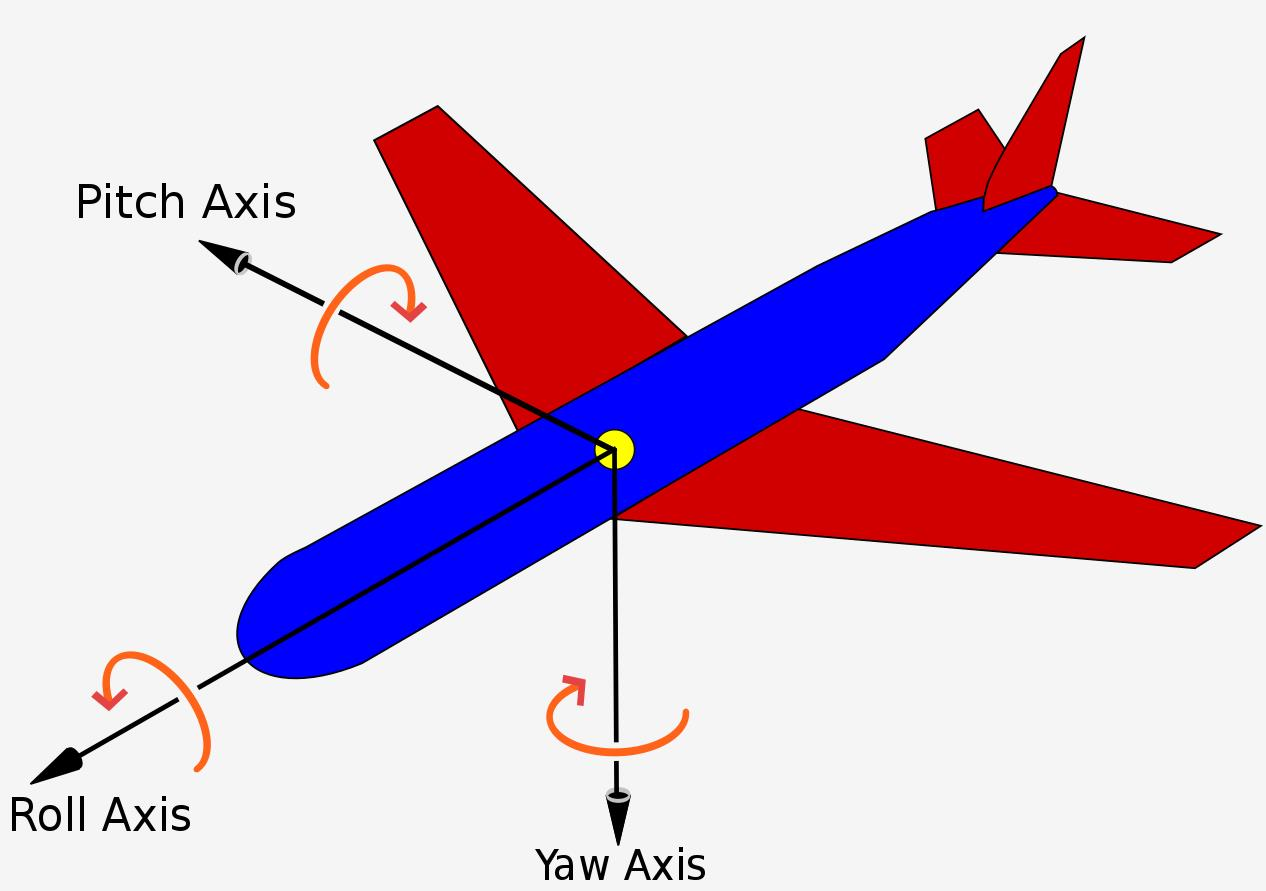
\includegraphics[width=0.6\textwidth]{images/2_2_roll_pitch_yaw}
    \caption{Roll-Pitch-Yaw axis representation.}\label{fig:euler-angles}
\end{figure}
So, by adding x,y, z axis as translations to three rotation angles ($\phi$, $\theta$, $\psi$) we can represent the pose of the camera in the world frame by using six numbers.
\subsubsection*{Roto-translation matrix}
In linear algebra, a \textit{roto-translation matrix} is a matrix that represents a rigid-body transformation.
It's called \textit{roto-translation} because it can be decomposed into a \textit{rotation matrix} and a \textit{translation}.

In details, the rotation matrix is defined as:
\begin{equation}
    \textbf{R} = \begin{bmatrix}
                     r_{11} & r_{12} & r_{13} \\
                     r_{21} & r_{22} & r_{23} \\
                     r_{31} & r_{32} & r_{33}
    \end{bmatrix}
    \label{eq:rotation_matrix}
\end{equation}
And it has the following properties:
\begin{itemize}
    \item It must be a square matrix.
    \item $\textbf{R}^T = \textbf{R}^{-1}$: the transpose of the rotation matrix is the inverse of the rotation matrix;
    \item $\textbf{R}^T \textbf{R} = \textbf{I}$: the transpose of the rotation matrix multiplied by the rotation matrix is the identity matrix;
    \item Multiplication of rotation matrices will result in a rotation matrix.
    \item The dot product of a row with column will be equal to 1.
    \item The cross product of two rows of a rotation matrix will be equal to the third row.
\end{itemize}
The translation vector is defined as:
\begin{equation}
    \textbf{t} = \begin{bmatrix}
                     t_{1} \\
                     t_{2} \\
                     t_{3}
    \end{bmatrix}
    \label{eq:translation_vector}
\end{equation}
The translation vector indicates the position of the origin of the new coordinate system with respect to the old one.
So, by combining rotation matrix and the translation vector, we will obtain:
\begin{equation}
    \textbf{A} = \begin{bmatrix}
                     r_{11} & r_{12} & r_{13} &t_{1}\\
                     r_{21} & r_{22} & r_{23} &t_{2}\\
                     r_{31} & r_{32} & r_{33} &t_{3}\\
                     0 & 0 & 0 & 1
    \end{bmatrix}
    \label{eq:roto-transformation}
\end{equation}
But, as the last row is always the same, we can ignore it, so we can write it as a sequence of 12 numbers like: $[r_{11}, r_{12}, r_{13}, t_{1}, r_{21}, r_{22}, r_{23}, t_{2}, r_{31}, r_{32}, r_{33}, t_{3}]$.
And this is the format that the KITTI dataset provides.

\subsection{Conversions}\label{subsec:conversions}
We mainly use two different representations of the pose of the camera, the \textit{Euler angles} and the \textit{roto-translation matrix}.
So we need to convert from Euler angles to the roto-translation matrix and back.

\subsubsection*{Euler angles to roto-translation matrix}
To compute the roto-translation matrix, we need to compute the rotation matrix meanwhile the translation vector is already provided.
To compute the rotation matrix, we need to compute the rotation matrix for each axis, then we need to multiply them.
The rotation matrix for the \textit{roll} axis is defined as:
\begin{equation}
    \textbf{R}_{roll} = \begin{bmatrix}
                     1 & 0 & 0 \\
                     0 & \cos(\phi) & -\sin(\phi) \\
                     0 & \sin(\phi) & \cos(\phi)
    \end{bmatrix}
    \label{eq:rotation_matrix_roll}
\end{equation}
The rotation matrix for the \textit{pitch} axis is defined as:
\begin{equation}
    \textbf{R}_{pitch} = \begin{bmatrix}
                     \cos(\theta) & 0 & \sin(\theta) \\
                     0 & 1 & 0 \\
                     -\sin(\theta) & 0 & \cos(\theta)
    \end{bmatrix}
    \label{eq:rotation_matrix_pitch}
\end{equation}
The rotation matrix for the \textit{yaw} axis is defined as:
\begin{equation}
    \textbf{R}_{yaw} = \begin{bmatrix}
                     \cos(\psi) & -\sin(\psi) & 0 \\
                     \sin(\psi) & \cos(\psi) & 0 \\
                     0 & 0 & 1
    \end{bmatrix}
    \label{eq:rotation_matrix_yaw}
\end{equation}
So, the rotation matrix is defined as:
\begin{equation}
    \textbf{R} = \textbf{R}_{roll} \textbf{R}_{pitch} \textbf{R}_{yaw}
    \label{eq:eq-rotation_matrix}
\end{equation}
Then, by concatenating the translation matrix and the rotation matrix, we will obtain the roto-translation matrix.
\subsubsection*{Roto-translation matrix to Euler angles}
To compute the Euler angles, we need only the rotation matrix, then we need to extract each euler angle from it.
So, given a rotation matrix as the equation 2.5, the three Euler angles are:
\begin{enumerate}
    \item $\phi = \arctan2(r_{32}, r_{33})$
    \item $\theta = \arctan2(-r_{31}, \sqrt{r_{32}^2 + r_{33}^2})$
    \item $\psi = \arctan2(r_{21}, r_{11})$
\end{enumerate}
Here, $\arctan2$ is the same arc-tangent function, with quadrant checking.

\subsection{State of the art}\label{subsec:state-of-the-art}
With the development of machine-learning tools, as the~(\cite{vo_state_of_art}) introduces, the recent years have seen a lot of researchers to tackle the VO problem with deep learning.
This approach has an important advantage which the fact that it can be done without prior knowledge of the camera parameters.
An example fo the earliest work on learning-based VO divided the image into blocks, then, they developed a k-NN regression model that was trained to compute the optimal flow for each block.
A second proposal is to estimate the \gls{opticalflow} by a linear subspace if there were considerable depth regularities relative to the robot motion in the environment.

The successive proposals are mainly based on CNN, and they are based on a depth-estimation and motion-estimation across image pairs.
Then, they used the same networks to estimate the local velocity and its direction.

The recurrent CNN was developed for pose estimation in an end-to-end manner.
Furthermore, CNN model was developed using monocular vision to estimate the vehicle's position in a true scale.

With monocular visual odometry we need to combine CNN and Bi-LSTM to leverage the feature properties of image pairs and to permit understanding  of the relationship between the features of successive images.
Another solution could be to use the R-CNN employing RGB-D sensors.
By including the depth information, inferring an accurate pose from monocular images.
Recently, Wang et al.~(\cite{wang_vo}) exploited a solution based on deep siamese convolutional neural network (DSCNN) and the second one called DL-based Monocular which depends on the first network.
The DSCNN model then is trained by the geometrical relationship of consecutive images to find a 6-DoF pose.
For more details about the current state-of-the-art, please refer to~\cite{vo_state_of_art}.

\subsection{Metrics}\label{subsec:ate-and-rte}
As presented by Prokhorov et al.~(\cite{measuring_robustness_of_visual_slam}), we can measure the global consistency of the trajectory by comparing the absolute distances between estimated and ground truth trajectory.
As both trajectories can be specified in arbitrary coordinate frames, they first need to be aligned.
Then, we should define the absolute trajectory error matrix at time $i$ as:
\begin{equation}
    \label{eq:ate-error-matrix}
    E_i \coloneq Q_i^{-1} SP_i
\end{equation}
Where S is the rigid-body transformation found by Horn Method (Horn et al.\cite{horn_method}).
Then, the ATE is defined as the root-mean-square error from error matrices:
\begin{equation}
    ATE_{rmse} = (\frac{1}{n} \sum_{i=1}^{n} ||E_i||^2)^{1/2}
    \label{eq:ate-rmse}
\end{equation}
The relative pose error measure is the local accuracy of the trajectory over a fixed time interval $\Delta$.
Therefore, the RTE corresponds to the drift of the trajectory which is in particular useful for the evaluation of visual odometry systems.
The RTE is defined as follows:
\begin{equation}
    F_i^{\Delta} \coloneq (Q_i^{-1} Q_{i+\Delta})^{-1} (P_i^{-1} P_{i+\Delta})
    \label{eq:rte}
\end{equation}
from a sequence of $n$ camera poses we obtain  $m = n - \Delta$ individual relative pose error matrices along the sequence.
The RPE is usually divided into translation component and rotation component.
Similarly to ATE, we can compute the root-mean-square error over all time indices for RPE translation error:
\begin{equation}
    RPE_{trans}^{i, \Delta} \coloneq (\frac{1}{m} \sum_{i=1}^m ||trans(F_i)||^2)^{½}
    \label{eq:rpe-trans}
\end{equation}
And for the rotation component we use mean error approach:
\begin{equation}
    RPE_{trans}^{i, \Delta} \coloneq \frac{1}{m} \sum_{i=1}^m \angle (rot(F_i^\Delta))
    \label{eq:equation-rpe-trans}
\end{equation}